% Partie 3: l'héritage
\chapter{La maladie, la mort, l'héritage}
\epigraph{BONNE NUIT, L'OURS, ET MON PAT, ET MA LALA. TROIS QUE J'AIME. BONNE NUIT BEAUCOUP D'AUTRES. J'EN AIME BEAUCOUP D'AUTRES. C'EST JOLI DE VIVRE. J'AIME BIEN AUSSI.}
{\BV}
\epigraph{\ldots Comme tout le monde, je passe ma vie à préparer une image déformée du cadavre
que je serai, comme s'il n'allait pas se déformer suffisamment tout seul.}
{\emph{Lettre à Jacques Bens}, \nb{15} juin \nb{1959}}
\vfill
\pagebreak
\section{La maladie}
\epigraph{Le temps, le temps, il me cavale au cul comme une charge de uhlans; et le c\oe{}ur qui me gène\ldots}
{\BV, le \nb{26} février \nb{1956}}

\lettrine{L}a maladie, Boris l'a toujours connue. Plus que cela, il a vécu avec. L'a vécue, même.
Elle a commencé à le couvrir de son aile sombre dès son plus jeune âge: à \nb{12} ans, il
est victime d'une angine infectieuse. S'en suit une insuffisance aortique, provoquée 
par des rhumatismes articulaires aigus.

Puis, au cours de sa (courte) vie, elle s'est rappelée à son bon souvenir
avec plus ou moins de véhémence, le forçant à se médicamenter sans relâche. En juillet, belote \nb{1956},
les choses se précipitent lorsqu'il est victime d'un \oe{}dème pulmonaire.
En septembre \nb{1957}, c'est re-belote. Le \nb{10} de der' a été remporté par la maladie
en 1959, après deux années qui ont vu Boris se fatiguer de plus en plus.

\subsection{La souffrance}
Il est facile d'imaginer que cette maladie a fait souffrir \BV. Il est
pourtant beaucoup plus difficile de mesurer précisément l'ampleur de
cette souffrance.

\subsubsection{Le renoncement}
Un des indicateurs les plus représentatifs, pourrait être donné par son amour
pour le jazz, en particulier de \emph{jouer} du jazz sur sa trompinette.

À cause de cette insuffisance aortique, il est obligé de mettre en sourdine\footnote{C'est le cas
de le dire\ldots} sa carrière de musicien amateur, puis, cédant aux médecins, de l'arrêter
définitivement. Chaque tentative de reprise se soldait par un gravement de son état de santé.
Il en est conscient\~: «Chaque souffle dans ma trompette abrège mes jours». Les journalistes à
qui il annonce cela ne le prennent pas au sérieux. On attend rien de sérieux d'un
amuseur comme Boris.

De trompette dans l'orchestre de Claude \bsc{Abadie}, il ne joue plus que ponctuellement avec des
formations musicales. Il anime cependant, mais usant de la trompinette avec parcimonie
\footnote{Qui n'est pourtant pas sa grande amie, on l'aura compris}, les nuit de Saint-Germain-des-Prés.

Ce renoncement se fait dans la douleur, le fait qu'il ait continué en se sachant malade montrant
combien il ne voulait pas abandonner. La Raison l'a cependant emporté. Mort, il est beaucoup
plus difficile d'accomplir les «mille choses» qu'il se sent en mesure de réaliser.

\subsubsection{La négation et la fuite en avant}

Quel rôle a joué la maladie sur Boris ? En lui donnant une durée de vie limitée, cela
ne l'a-t-il pas poussé dans ses derniers retranchements, l'obligeant à \emph{tout} faire
avant qu'il ne soit trop tard ? Noël \bsc{Arnaud} décrit son état d'esprit:
{\small
\begin{quotation}
L'attitude psychologique de \BV\ devant la maladie se caractérisait par deux éléments
contradictoires: a) il avait conscience d'être atteint d'une affection grave et il soupçonnait que
que son temps était limité [\ldots]; b) il n'acceptait pas cette situation et il s'efforçait de se
prouver à lui-même qu'il pouvait mener une vie normale. On serait tenté de parler d'une
véritable fuite devant la maladie; c'était plutôt une négation.
\end{quotation}
}
Pour illustrer cet état d'esprit auto-destructeur, voilà ce qu'aurait dit
Boris à un ami lui faisant remarquer son teint «endive»:
{\small
\begin{quotation}
Quand tu as une bagnole qui tousse, tu lui fous trois ou quatre coups d'accélérateurs,
et après ça tourne rond.
\end{quotation}
}
C'était deux jours avant sa mort subite.


\subsection{Dans son \oe{}uvre}

\subsubsection{L'herbe rouge}
Dans \emph{L'herbe rouge}, le personnage principal, Wolf, parle de son histoire, de son enfance
avec un personnage chargé de passer sa vie en revue, M. Perle.
Cette enfance ressemble a s'y méprendre à celle de \BV, surprotégé
par sa mère, enfermé dans un environnement sûr, toujours sous la main, en témoigne la
salle de réception construite par le père pour ne pas que la fratrie aie besoin de faire
la fête ailleurs.

{\small
\begin{quotation}
Ils avaient toujours peur pour moi, dit Wolf. Je ne pou­vais pas me pencher aux fenêtres,
je ne traversais pas la rue tout seul, il suffi­sait qu'il y ait un peu de vent pour qu'on
me mette ma peau de bique et hiver comme été, je ne quittais pas mon gilet en laine ;
c’étaient des tricots jaunâtres et distendus qu’on nous faisait avec de la laine de pays.
Ma santé, c’était effrayant. Jus­qu’à quinze ans je n’ai pas eu le droit de boire autre chose
que de l’eau bouillie. Mais la lâcheté de mes parents, c’est qu’eux-mêmes ne se ménageaient
pas et se donnaient tort dans leur conduite à mon égard par leur comportement envers eux-mêmes.
À force, je finis­sais par avoir peur moi-même, par me dire que j’étais très fragile, et j’étais
presque content de me promener, en hiver, en transpirant dans douze cache-nez de laine. Pendant
toute mon enfance, mon Père et ma Mère ont pris sur eux de m’épargner tout ce qui pouvait me
heurter. Mo­ra­le­ment, je ressentais une gêne vague, mais ma chair molle s’en ré­jouis­sait
hypocritement.

{\bf \emph{L'herbe rouge}, chapitre XVI}
\end{quotation}
}


\subsubsection{L'écume des jours}
Le «nénuphar» de Chloé est l'un des thèmes principaux
de ce roman. La maladie, qu'il est possible de soulager de temps à autre,
progresse inéluctablement. Et cela, malgré tous les efforts, tous les
sacrifices des autres personnages. Elle provoque l'extinction lente
de Chloé, entraînant la dégradation du monde qui l'entoure.


{\small
\begin{quotation}
« Ça ne va pas ? » dit Nicolas sans se retourner, avant que la voiture démarre.

Chloé pleurait toujours dans la fourrure blanche et Colin avait l’air d’un homme mort. L’odeur des trottoirs montait de plus en plus. Les vapeurs d’éther emplissaient la rue.

« Va, dit Colin.

– Qu’est-ce qu’elle a ? demanda Nicolas.

– Oh ! Ça ne pouvait pas être pire ! » dit Colin.

Il se rendit compte de ce qu’il venait de dire et regarda Chloé. Il l’aimait tellement en ce moment qu’il se serait tué pour son imprudence.

Chloé, recroquevillée dans un coin de la voiture, mordait ses poings. Ses cheveux lustrés lui tombaient sur la figure et elle piétinait sa toque de fourrure. Elle pleurait de toutes ses forces, comme un bébé, mais sans bruit.

« Pardonne-moi, ma Chloé, dit Colin. Je suis un monstre. »

Il se rapprocha d’elle et la prit près de lui. Il embrassait ses pauvres yeux affolés et sentait son cœur battre à coups sourds et lents dans sa poitrine.

« On va te guérir, dit-il. Ce que je voulais dire, c’est qu’il ne pouvait rien arriver de pire que de te voir malade quelle que soit la maladie…

– J’ai peur… dit Chloé. Il m’opérera sûrement.

– Non, dit Colin. Tu seras guérie avant.

– Qu’est-ce qu’elle a ? répéta Nicolas. Je peux faire quelque chose ? »

Lui aussi avait l’air très malheureux. Son aplomb ordinaire s’était fortement ramolli.

« Ma Chloé, dit Colin, calme-toi.

– C’est sûr, dit Nicolas. Elle sera guérie très vite.

– Ce nénuphar, dit Colin. Où a-t-elle pu attraper ça ?

– Elle a un nénuphar ? demanda Nicolas incrédule.

– Dans le poumon droit, dit Colin. Le professeur croyait au début que c’était seulement quelque chose d’animal. Mais c’est ça. On l’a vu sur l’écran. Il est déjà assez grand, mais, enfin, on doit pouvoir en venir à bout.

– Mais oui, dit Nicolas.

– Vous ne pouvez pas savoir ce que c’est, sanglota Chloé, ça fait tellement mal quand il bouge ! ! !

– Pleurez pas, dit Nicolas. Ça sert à rien et vous allez vous fatiguer. »

{\bf \emph{L'écume des jours}, chapitre XL}
\end{quotation}
}

Dans cette \oe{}uvre encore se tisse un parallèle entre un personnage du livre et
\BV.


\section{La mort}
\epigraph{%
J'suis snob... Encore plus snob que tout à l'heure\\%
Et quand je serai mort\\%
J'veux un suaire de chez Dior !%
}{\emph{J'suis snob}, Boris Vian}

\lettrine{J}e ne sais pas si \BV\ a été enterré dans un suaire de chez Dior,
comme il le réclamait dans sa chanson «J'suis snob»\ldots ça aurait été la
moindre des choses. Enfin, je ne suis pas tout à fait persuadé que Dior
ai développé une ligne de suaires. Ils auraient pu commencer avec celui
de Boris\ldots

\subsection{La malédiction}
L'ayant poursuivi dès sa création, \emph{J'irai cracher sur vos tombes}, à
l'origine une bonne blague, l'aura finalement achevé. Ironie finie, quand
on sait qu'il est mort d'une crise cardiaque lors de la première
projection d'une adaptation de son \oe{}uvre qu'il avait tout fait pour
qu'elle ne voie pas le jour. Las. Par une vengeance d'une bassesse innommable,
celle ci n'a pas attendu les premières minutes pour porter le coup fatal.

\subsection{Dans son \oe{}uvre}
Se sachant condamné, \BV\ vit à cent à l'heure, accomplissant plus en \nb{39} ans
d'existence que ce que l'on pourrait imaginer réaliser en \nb{80}. Son \oe{}uvre 
est bien sûr marquée par cette menace de moins en moins diffuse à mesure que 
les années passent, et que les problèmes de santé se multiplient. «Je ne
vivrai pas jusqu'à \nb{40} ans», a-t-il dit un jour\footnote{D'après Noël \bsc{Arnaud}, dans \emph{Les vies parallèles de Boris Vian}, il n'aurait pas appris cela de la bouche d'un médecin, mais aurait pu réaliser le pronostic lui-même en se documentant par ses propres moyens.}. On en vient presque à
regretter tant de clairvoyance. Cependant, ses amis savaient que ses jours
étaient comptés. Ainsi, ils avaient conscience que chaque note qui sortait
de sa trompinette le rapprochait un peu plus de la tombe. Pourtant, il
s'efforçait de vivre, le plus intensément possible.

Sa mort ne venant pas par surprise --- seule la date exacte,
judicieusement choisie par le Sort, ça l'aurait probablement fait rire,
a été gardée secrète jusqu'au bout; il a eu le temps d'y réfléchir. Il y
fait référence dans beaucoup de ses textes. Voilà une petite sélection,
pour se faire une idée.

\subsubsection{Quand j'aurai du vent dans mon crâne}

Il s'agit d'une chanson
(je ne peux malheureusement pas inclure dans ce document
la très bonne interprétation de Serge \bsc{Reggiani}, je vais donc simplement
en recommander fortement l'écoute), sur une musique de l'inénarrable Serge \bsc{Gainsbourg}.

\begin{multicols}{2}
{\footnotesize
\settowidth{\versewidth}{Quand j'aurai du vent dans mon crâne}
\begin{verse}[\versewidth]
Quand j'aurai du vent dans mon crâne\\
Quand j'aurai du vert sur mes osses\\
P'tet qu'on croira que je ricane\\
Mais ça sera une impression fosse\\
Car il me manquera\\
Mon élément plastique\\
Plastique tique tique\\
Qu'auront bouffé les rats\\
Ma paire de bidules\\
Mes mollets mes rotules\\
Mes cuisses et mon cule\\
Sur quoi je m'asseyois\\
Mes cheveux mes fistules\\
Mes jolis yeux cérules\\
Mes couvre-mandibules\\
Dont je vous pourléchois\\
Mon nez considérable\\
Mon coeur mon foie mon râble\\
Tous ces riens admirables\\
Qui m'ont fait apprécier\\
Des ducs et des duchesses\\
Des papes des papesses\\
Des abbés des ânesses\\
Et des gens du métier\\
Et puis je n'aurai plus\\
Ce phosphore un peu mou\\
Cerveau qui me servit\\
A me prévoir sans vie\\
Les osses tout verts, le crâne venteux\\
Ah comme j'ai mal de devenir vieux.


\end{verse}
}
\end{multicols}

En parlant d'interprétation, je ne peux m'empêcher d'inclure ici la version
du dessinateur de bande dessinée Boulet, publiée sur son blog à l'occasion
de son trente et unième anniversaire. Un très bel hommage, respectant
d'après moi l'esprit de la chanson, à lire en fig. \ref{boulet}%
--- que j'ai malheureusement dû couper pour passer du format «Internet» au format «livre».

\begin{figure}[!htb]
\centering
\begin{subfigure}[b]{\textwidth}
%\subfloat[][]{%
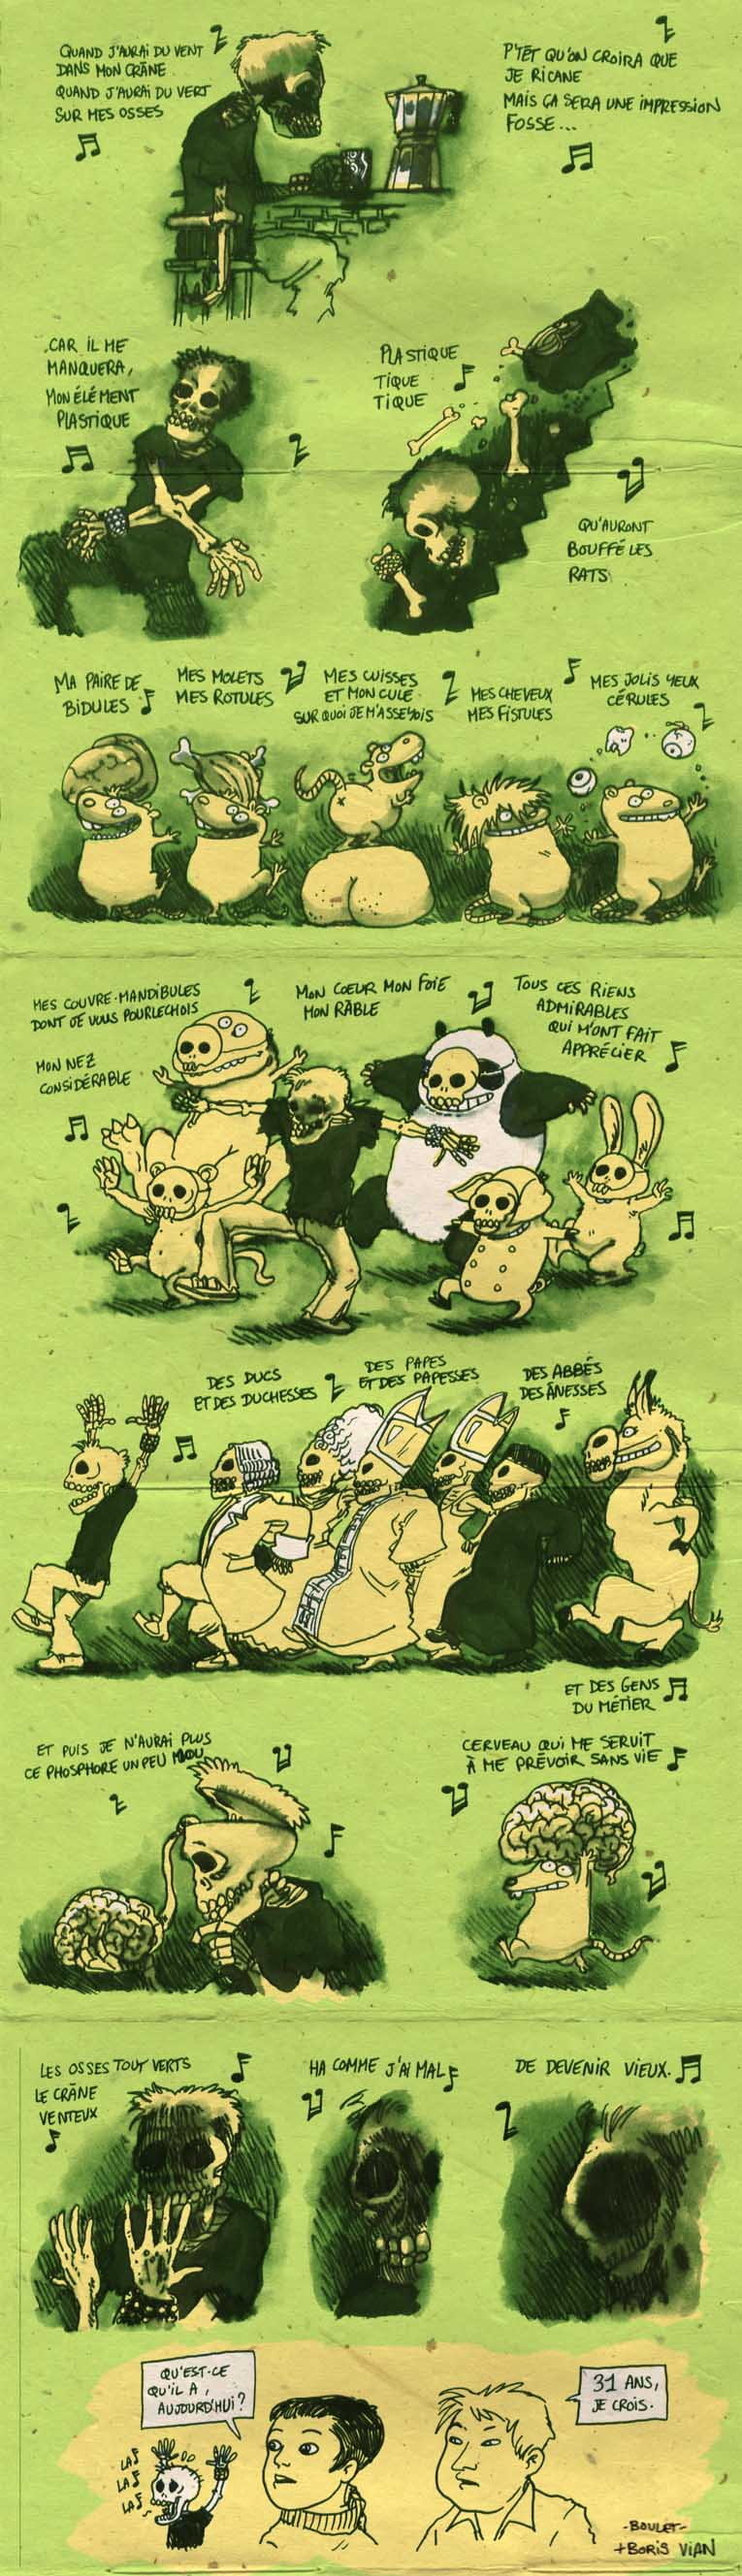
\includegraphics[trim=0cm 337mm 0cm 0cm, clip]{\PIXPATH/bouletbison}%
%\caption{Première partie}
\end{subfigure}
%}
\caption{\emph{Bison Ravi}, note de Boulet du \nb{31} janvier \nb{2006}}
\label{boulet}
\end{figure}
\begin{figure}[!htb]
\ContinuedFloat
\centering
\begin{subfigure}[b]{\textwidth}
%\subfloat[][]{%
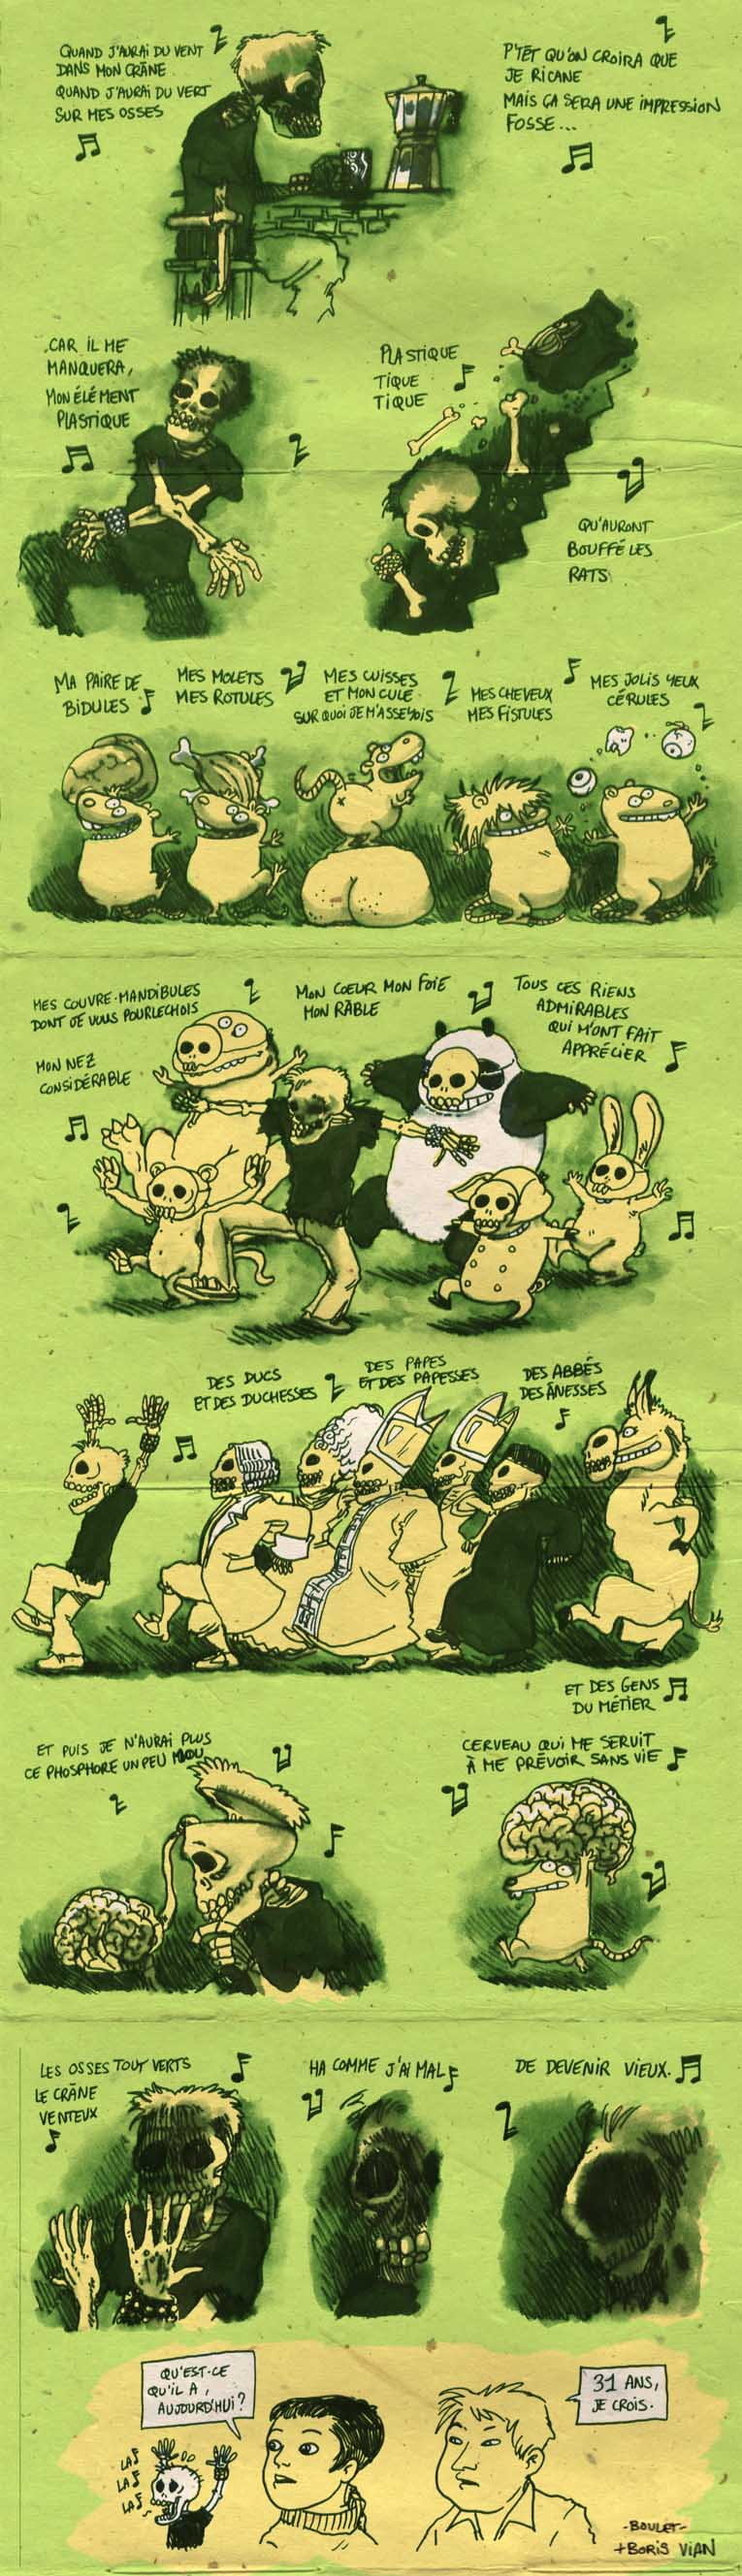
\includegraphics[trim=0cm 148mm 0cm 113mm, clip]{\PIXPATH/bouletbison}%
%\caption{Seconde partie}
%\caption{Première partie}
\end{subfigure}
\caption{\emph{Bison Ravi}, note de Boulet du \nb{31} janvier \nb{2006}}
\label{boulet}
\end{figure}
\eject
\begin{figure}[!htb]
\ContinuedFloat
\centering
\begin{subfigure}[b]{\textwidth}
%\subfloat[][]{%
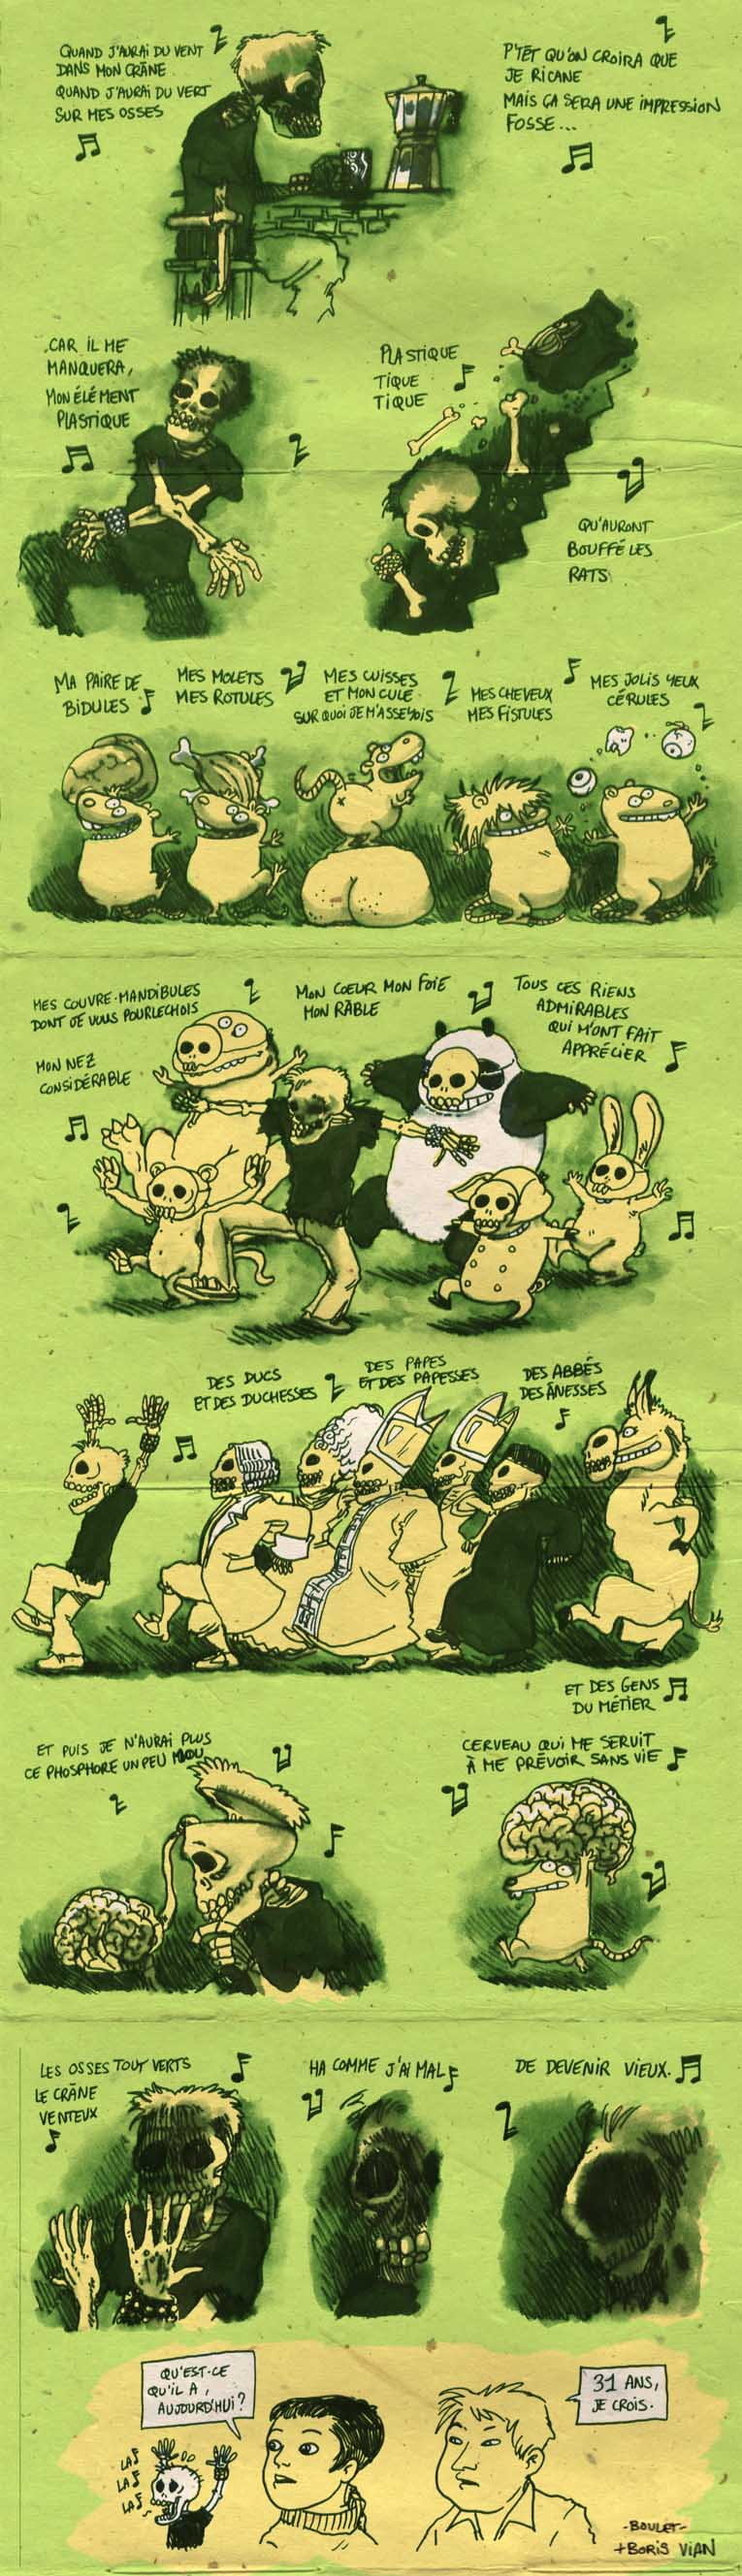
\includegraphics[trim=0cm 0mm 0cm 300mm, clip]{\PIXPATH/bouletbison}%
%\caption{Seconde partie}
%}
\end{subfigure}
\caption{\emph{Bison Ravi}, note de Boulet du \nb{31} janvier \nb{2006}}
\label{boulet}
\end{figure}
\eject
\FloatBarrier

\subsubsection{Je voudrais pas crever}
Il s'agit d'un poème écrit vers \nb{1951}, quand il vit déjà avec Ursula
\bsc{Kubler}(son «ourson»). On ressent sans peine l'envie de vivre de
l'auteur, qui sait pertinemment qu'il ne vivra pas assez longtemps pour
tout ce qu'il aimerait faire et voir.

\begin{multicols}{2}
{\footnotesize
\settowidth{\versewidth}{Où valsent les brins d'algues}
\begin{verse}
Je voudrais pas crever\\
Avant d'avoir connu\\
Les chiens noirs du Mexique\\
Qui dorment sans rêver\\
Les singes à cul nu\\
Dévoreurs de tropiques\\
Les araignées d'argent\\
Au nid truffé de bulles\\
Je voudrais pas crever\\
Sans savoir si la lune\\
Sous son faux air de thune\\
A un coté pointu\\
Si le soleil est froid\\
Si les quatre saisons\\
Ne sont vraiment que quatre\\
Sans avoir essayé\\
De porter une robe\\
Sur les grands boulevards\\
Sans avoir regardé\\
Dans un regard d'égout\\
Sans avoir mis mon zobe\\
Dans des coinstots bizarres\\
Je voudrais pas finir\\
Sans connaître la lèpre\\
Ou les sept maladies\\
Qu'on attrape là-bas\\
Le bon ni le mauvais\\
Ne me feraient de peine\\
Si si si je savais\\
Que j'en aurai l'étrenne\\
Et il y a z aussi\\
Tout ce que je connais\\
Tout ce que j'apprécie\\
Que je sais qui me plaît\\
Le fond vert de la mer\\
Où valsent les brins d'algues\\
Sur le sable ondulé\\
L'herbe grillée de juin\\
La terre qui craquelle\\
L'odeur des conifères\\
Et les baisers de celle\\
Que ceci que cela\\
La belle que voilà\\
Mon Ourson, l'Ursula\\
Je voudrais pas crever\\
Avant d'avoir usé\\
Sa bouche avec ma bouche\\
Son corps avec mes mains\\
Le reste avec mes yeux\\
J'en dis pas plus faut bien\\
Rester révérencieux\\
Je voudrais pas mourir\\
Sans qu'on ait inventé\\
Les roses éternelles\\
La journée de deux heures\\
La mer à la montagne\\
La montagne à la mer\\
La fin de la douleur\\
Les journaux en couleur\\
Tous les enfants contents\\
Et tant de trucs encore\\
Qui dorment dans les crânes\\
Des géniaux ingénieurs\\
Des jardiniers joviaux\\
Des soucieux socialistes\\
Des urbains urbanistes\\
Et des pensifs penseurs\\
Tant de choses à voir\\
A voir et à z-entendre\\
Tant de temps à attendre\\
A chercher dans le noir

Et moi je vois la fin\\
Qui grouille et qui s'amène\\
Avec sa gueule moche\\
Et qui m'ouvre ses bras\\
De grenouille bancroche

Je voudrais pas crever\\
Non monsieur non madame\\
Avant d'avoir tâté\\
Le goût qui me tourmente\\
Le goût qu'est le plus fort\\
Je voudrais pas crever\\
Avant d'avoir goûté\\
La saveur de la mort...


\end{verse}
}
\end{multicols}

J'ai intégré ce texte car je je trouve très fort et représentant bien ce sentiment de fin inéluctable et d'impuissance de \BV\ldots

J'ai pu écouter
deux très bonnes versions. La première est récitée par Jean \bsc{Rochefort} accompagné
par Claude \bsc{Luter} à la clarinette sur l'album \emph{Une heure passée avec \BV\ }
sorti en \nb{1987}; la seconde est récitée par Édouard \bsc{Baer} sur
l'album-hommage \emph{À \BV: On est pas là pour se faire engueuler !} sorti en \nb{2009}.

%\section{Un héritage riche et une influence encore vive aujourd'hui}
\section{Un héritage riche}

En ayant à l'esprit toutes (ou ne serait-ce même qu'une partie) des activités,
tous les métiers qu'il a exercé, il aurait été bien étonnant que \BV\ ne
laisse pas une trace, ne soit pas une source d'influences pour les générations
futures.
C'est effectivement le cas. Son héritage est riche et multiple, et je vais
développer ici les trois principaux aspects (il faut bien choisir) qui me semblent
les plus marquants de ces influences.

%\subsection{Culture et social}

\BV\ a laissé sa marque dans le paysage culturel et social français. Déjà
de son vivant, il marquait les esprits, étant un personnage un peu hors norme; et
certains de ces traits, en plus de ses \oe{}uvres, sont passés à la postérité.

%\paragraph{Le Prince de Saint-Germain}
\subsection{Saint-Germain}
\begin{wrapfigure}{r}{.5\textwidth}
\centering
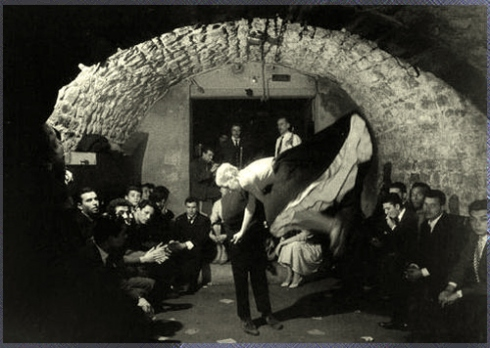
\includegraphics[width=.48\textwidth]{\PIXPATH/stgermain}
\caption{Dans une cave de St-Germain. Ici, le Caveau de la Huchette.}
\end{wrapfigure}
Qui n'a jamais entendu parler de Saint-Germain-des-Prés ? Je parle bien sûr
du Saint-Germain de l'après-guerre, le lieu de rencontre des intellectuels et
des artistes parisiens: Jean-Paul \bsc{Sartre}, Raymond \bsc{Queneau}, Jacques \bsc{Prévert}\ldots % TODO: citer plus
et bien d'autres. Le soir, la jeunesse du tout-Paris se retrouve dans les caves
des établissements du quartier, dansant (et buvant) toute la nuit au son jazz
noir-américain. Swing, rires et cuites garantis sur facture !


\begin{wrapfigure}{l}{.5\textwidth}
\centering
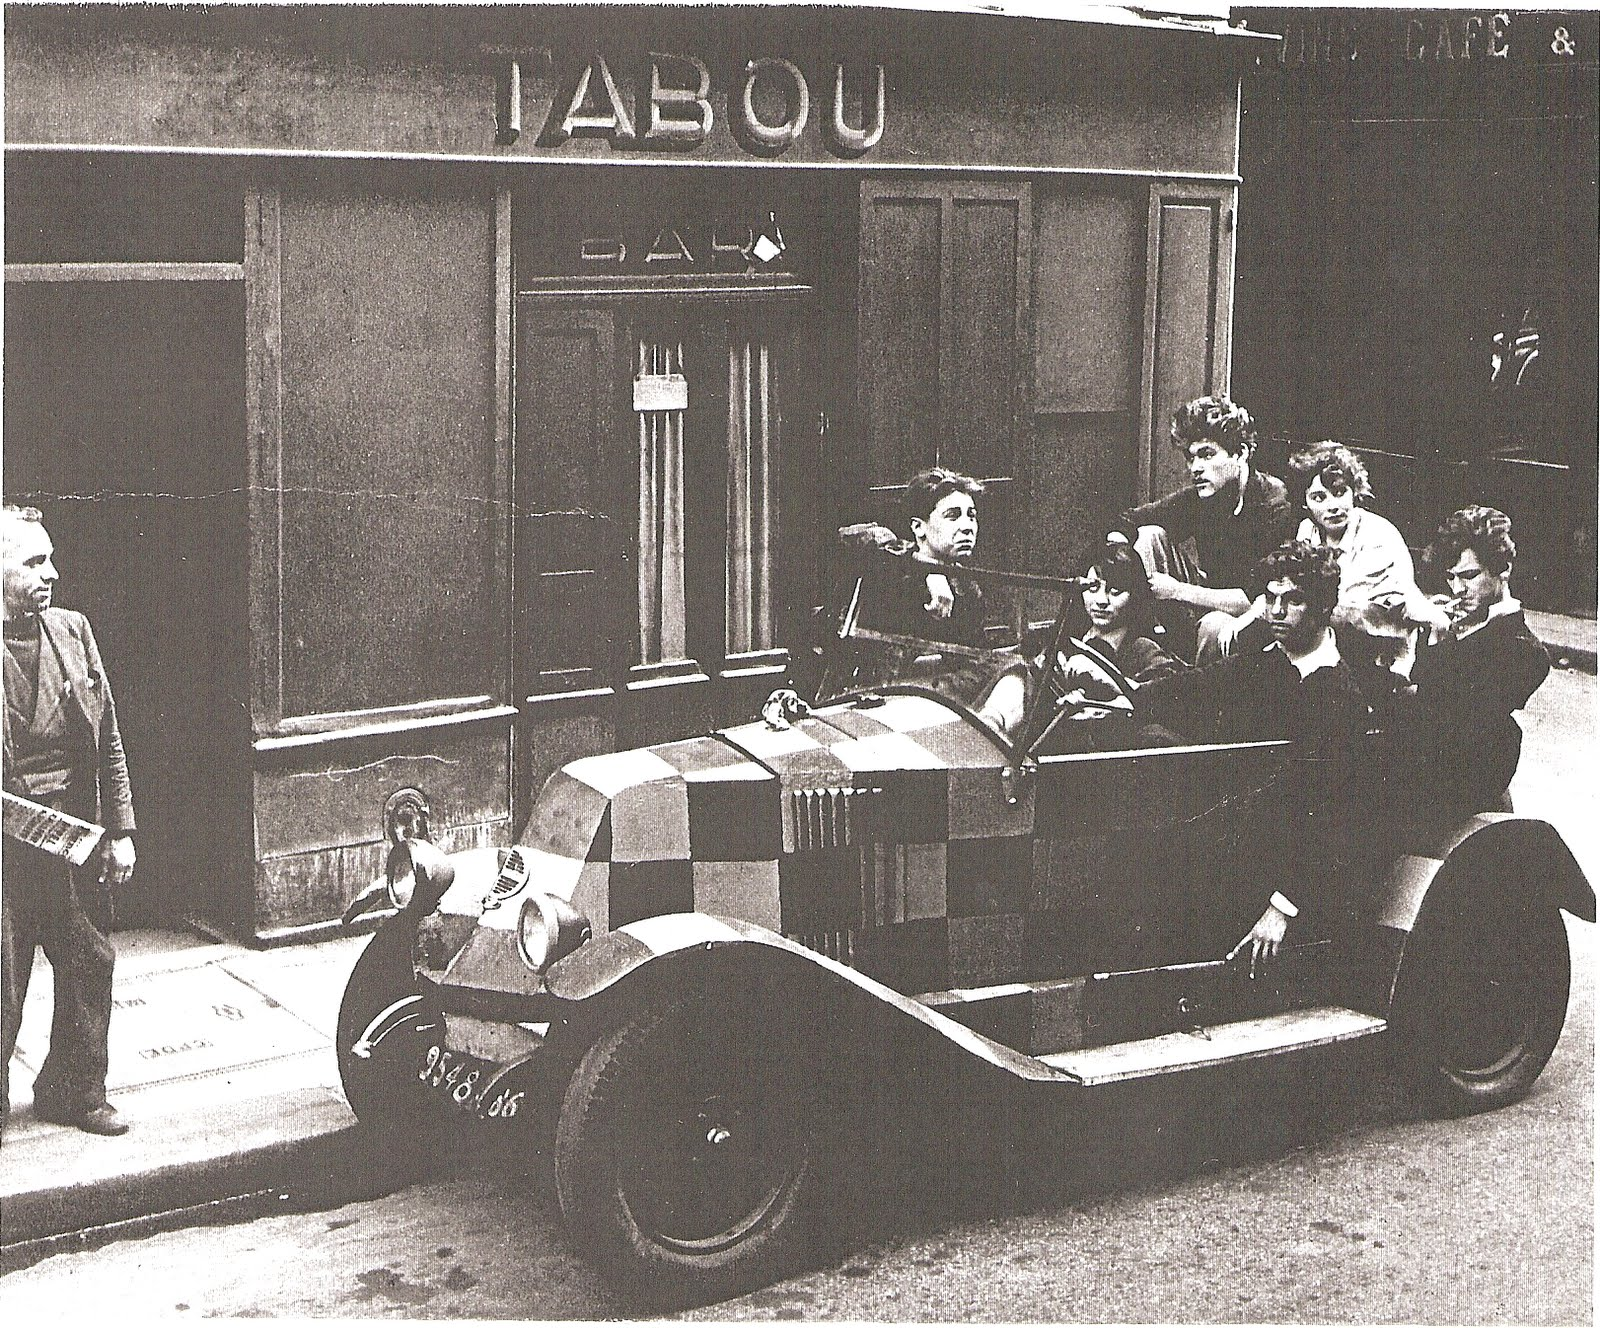
\includegraphics[width=.48\textwidth]{\PIXPATH/tabou}
\caption{Des zazous devant le Tabou.}
\end{wrapfigure}
Le surnom de «Prince de Saint-Germain» donné à \BV\ atteste de son importance
dans ce petit monde, connaissant tous (et toutes \ldots), animant avec ses amis et
ses frères les soirées endiablées, d'abord au \emph{Tabou}, puis une fois la
frénésie des premières années passées, dans l'ambiance plus feutrée du \emph{Club
Saint-Germain}.

Sa connaissance intime de Saint-Germain et de sa faune pousse un éditeur, au moment
ou Saint-Germain et les bacchanales qui s'y déroulent deviennent plus connues du
grand public, de demander au «Prince» un \emph{Manuel de Saint-Germain-des-Prés}.
L'ouvrage, prévu avec force descriptions farfelues et illustrations des gens et
lieux, ne fut hélas pas publié à l'époque\footnote{Il aura fallu attendre \nb{1974} et sa première (ré-)édition par les Éditions du Chêne pour cela. }, l'éditeur ayant fait faillite entre-temps.

\begin{figure}
\centering
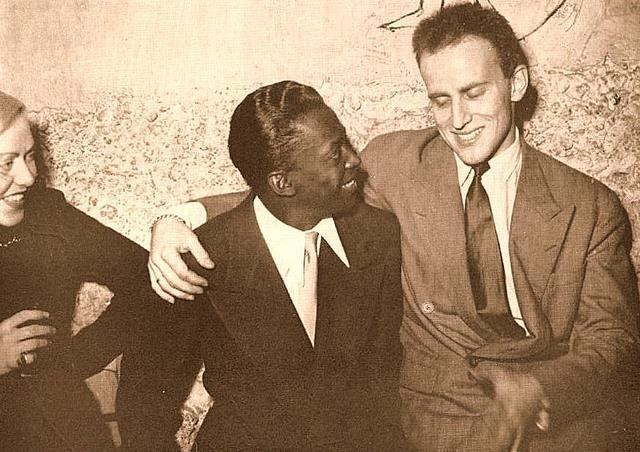
\includegraphics[width=.75\textwidth]{\PIXPATH/miles}
\caption{\BV\ et Miles \bsc{Davis}}
\end{figure}
C'est également dans ces clubs que \BV\ accueille ses idole du jazz que sont
Miles \bsc{Davis}, Duke \bsc{Ellington} (son dieu), et bien d'autres \ldots

%\paragraph{Langage}
\subsection{Langage}
Amateur de langage et de jeux de mots, expérimentateur du verbe et néologiste
patenté, écrivain et homme public: il n'est pas surprenant que des expressions
de son cru nous parviennent.
Le meilleur exemple est sans aucun doute l'utilisation du mot « tube ».

C'est lors d'une réunion de travail chez Philips en \nb{1957}, alors qu'il y ait
directeur artistique, qu'il propose ce mot pour désigner un succès populaire,
ou une chanson qui est assurée d'avoir du succès, parfois malgré l'ineptie du
texte ou la qualité musicale. Boris proposait ce mot pour remplacer l'alors
usité «saucisson». Devant la supériorité objective du candidat, il n'est pas
surprenant qu'il est été adopté --- difficile d'imaginer un \emph{disc jokey}
annoncer le dernier «saucisson» de l'été ! Par la même occasion, \BV\ a
fourni une alternative viable au \emph{hit} anglais. Cocorico.

%\paragraph{La génération \nb{68}}
\subsection{La génération \nb{68}}

\begin{wrapfigure}{R}{.30\textwidth}
\centering

\includegraphics[width=.25\textwidth]{\PIXPATH/ecumeroumain}
\caption{Édition roumaine de \emph{L'écume des jours}. Traduction de Sorin Mărculescu}
\label{eroum}
\end{wrapfigure}
La première large reconnaissance littérarité de \BV\ --- des œuvres signées
de son vrai nom s'entend --- fût apportée par la jeunesse de la fin des années \nb{60}.
Se sentant représentés par cet auteur si anticonformiste, anticonventionel, dont
le destin tragique à gonflé le mythe de rêveur à le jeunesse éternelle, \BV\ 
et son œuvre --- en particulier \emph{L'écume de jours} --- ont influencé toute une
génération. En avance sur son temps comme souvent --- même lorsqu'il s'agit de
mourir ! --- \BV\ n'a malheureusement pas connu cette gloire méritée.
Une gloire qui ne s'arrête d'ailleurs pas aux frontières de la France: \emph{L'écume
des jours} a été traduit dans plusieurs dizaines de langues, de l'anglais au japonais en passant
par le roumain (voir fig. \ref{eroum}).

%\paragraph{Postérité}
\subsection{Postérité}
Reconnu comme un auteur français incontournable, \BV\ est maintenant passé à la postérité.
Les collégiens étudient ses \oe{}uvres --- je n'ai malheureusement pas eu cette chance,
ce qui a retardé ma découverte de \BV; on trouve des établissements scolaires nommés en
son honneur (une rapide recherche Internet montre qu'il existe au moins 4 collèges \BV).

Sacrement suprême, son \oe{}uvre romanesque est publiée en \nb{2010} par Gallimard dans la collection
de la Pléiade. Boris rejoint ainsi le panthéon de la littérature française, \nb{50} ans après sa mort.

La Bibliothèque nationale de France à d'ailleurs, entre octobre 2011 et janvier \oldstylenums{2012}, présenté
une exposition sur BV\ (sobrement baptisée \emph{\BV}), où est retracé toute son histoire, où sont
représentées toutes ses facettes\footnote{Je n'ai malheureusement pas pu la visiter, effectuant un échange en Argentine à cette période\ldots quelle frustration ! Même si je ne regrette pour rien au monde cet échange, c'est tout de même rageant que cette évènement ait été organisé à ce moment là, j'aurais pu y consulter beaucoup de matériel pour ce PPH. Enfin, la vie est ainsi faite.}. Illustrée de plus de \oldstylenums{2000} documents originaux, cette
exposition montre que l'intérêt porté à \BV\ est loin de s'estomper. On pourrait même dire qu'il
grandit, en témoigne l'adaptation cinématographique de \emph{L'écume des jours} prévue pour \oldstylenums{2013}.
Réalisée par Michel \bsc{Gondry}, on pourra y voir Audrey \bsc{Tautou} donner la réplique à
Romain \bsc{Duris} et Gad \bsc{Elmaleh}. Rien que ça.

%\subsection{Musique}

%\subsection{Théâtre}


\section*{Conclusion}

On comprend maintenant pourquoi \BV\ vivait si intensément.

Pour tout faire avant qu'il ne soit trop tard,
il a produit, influencé, et les remous des cailloux qu'il a lancé nous parviennent encore, et ont
même tendance à s'amplifier, au fur et à mesure que son \oe{}uvre et son génie sont (re)découverts et appréciés.


